\documentclass{article}

\usepackage[utf8x]{inputenc}
\usepackage[english,russian]{babel}
\usepackage{cmap}
\usepackage{commath}
\usepackage{amsmath}
\usepackage{amsfonts}
\usepackage{mathtools}
\usepackage{amssymb}
\usepackage{parskip}
\usepackage{titling}
\usepackage{color}
\usepackage{hyperref}
\usepackage{cancel}
\usepackage{enumerate}
\usepackage{multicol}
\usepackage{graphicx}
\usepackage[font=small,labelfont=bf]{caption}
\usepackage[a4paper, left=2.5cm, right=1.5cm, top=2.5cm, bottom=2.5cm]{geometry}

\graphicspath{ {./images/} }
\setlength{\droptitle}{-3cm}
\hypersetup{ colorlinks=true, linktoc=all, linkcolor=blue }
\pagenumbering{arabic}

\begin{document}
    \section{Непрерывность функции в точке}

    \(a\) --- конечное число.

    \textbf{Определение.} Функция \(y = f(x)\) называется непрерывной в \(x = a\), если 

    \begin{enumerate}
        \item \(f(x)\) определена в \(U(a)\)
        \item \(lim_{x \rightarrow a} f(x) = f(a)\)
        
        Подробнее:

        \( \forall \varepsilon > 0\ \exists \delta(\varepsilon):\ \forall x:\ \abs{x - a} < \delta \Rightarrow \abs{f(x) - f(a)} < \varepsilon \)

        \(\exists \varepsilon:\ \forall \delta\ \exists x:\ \abs{x-a}<\delta\ \abs{f(x)-f(a)} \geq \varepsilon\)
    \end{enumerate}

    \begin{minipage}{0.49\linewidth}
        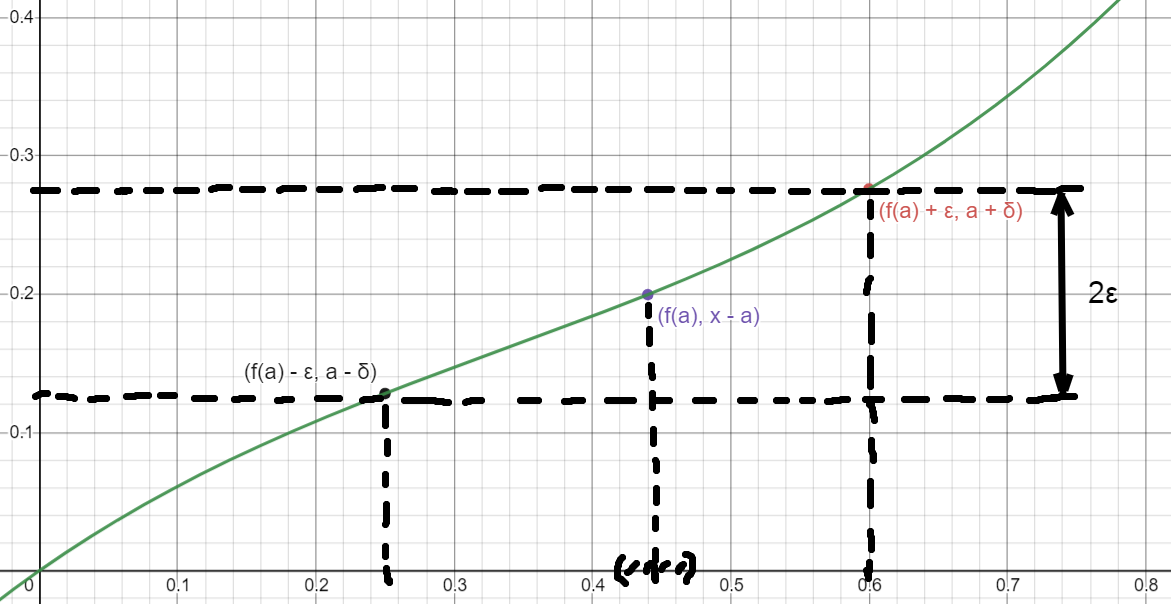
\includegraphics[scale=0.32]{11_1_3_1.png}
        \captionof{figure}{Пример неразрывности}
    \end{minipage}

    \subsection{Классификация точек разрыва}
    \(lim_{x \rightarrow a + 0} f(x) = A\)\\
    \(lim_{x \rightarrow a - 0} f(x) = A\)
    
    \textbf{Определение.} Функция \(y = f(x)\) называется непрерывной слева в \(x = a\), если

    \begin{enumerate}
        \item \(f(x)\) определена \( \forall x \in (a - \delta; a] \)
        \item \(lim_{x\rightarrow a-0} f(x)=f(a)\)
    \end{enumerate}

    \textbf{Определение.} Функция \(y = f(x)\) называется непрерывной справа в \(x = a\), если
    
    \begin{enumerate}
        \item \(f(x)\) определена \( \forall x \in [a; a + \delta) \)
        \item \(lim_{x\rightarrow a+0} f(x)=f(a)\)
    \end{enumerate}

    Понятно, что \( lim_{x \rightarrow a} f(x) = f(a) \Leftrightarrow lim_{x \rightarrow a + 0} f(x) = f(a) = lim_{x \rightarrow a - 0} f(x) \)

    \textbf{Определение.} Если существуют конечные пределы \(lim_{x \rightarrow a+0} f(x)\) и \(lim_{x \rightarrow a-0} f(x)\), но функция разрывна, то в \(x=a\) разрыв 1-го рода.

    \(y=\begin{cases}\frac{x^2-4}{x-2}\\ 4;\ x=2\end{cases}\)

    \begin{minipage}{0.49\linewidth}
        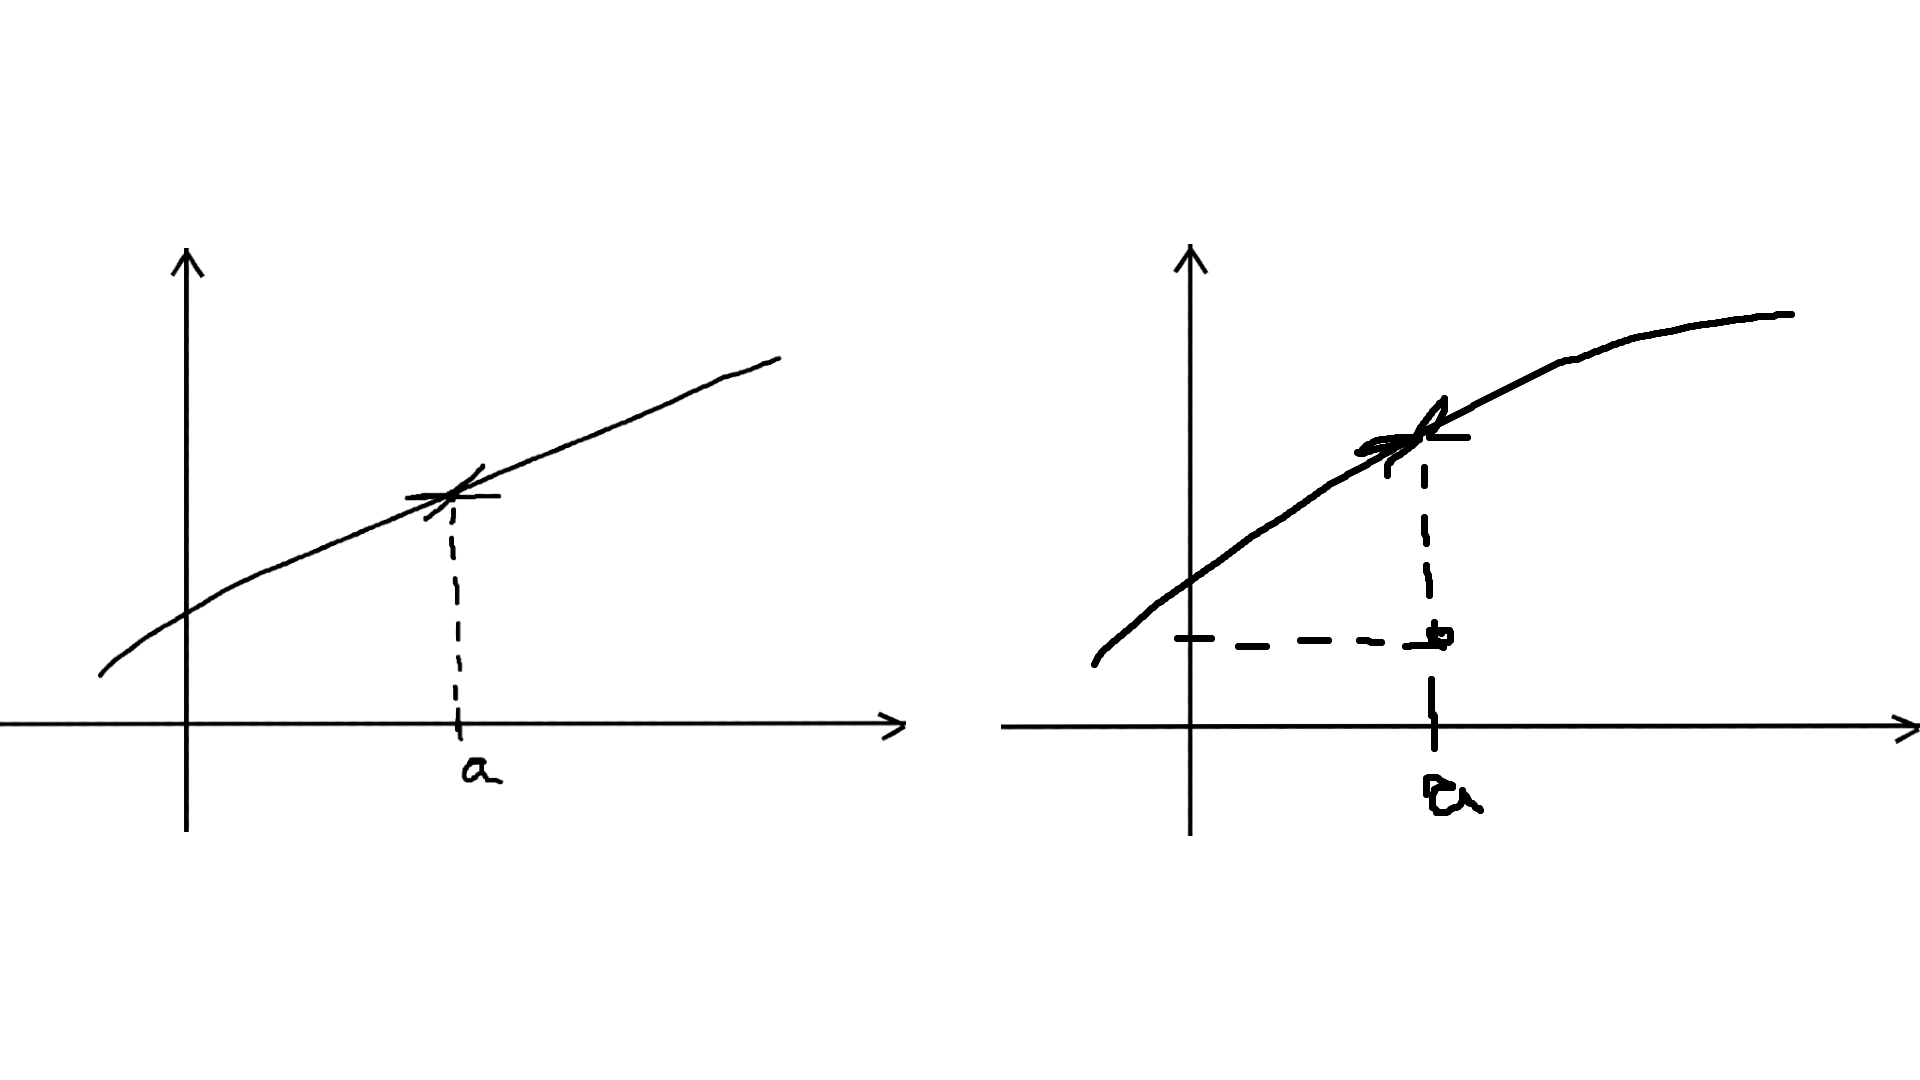
\includegraphics[trim={0 9cm 0 9cm},clip, width=\linewidth]{11_1_3_2.png}
        \captionof{figure}{Устранимые разрывности}

        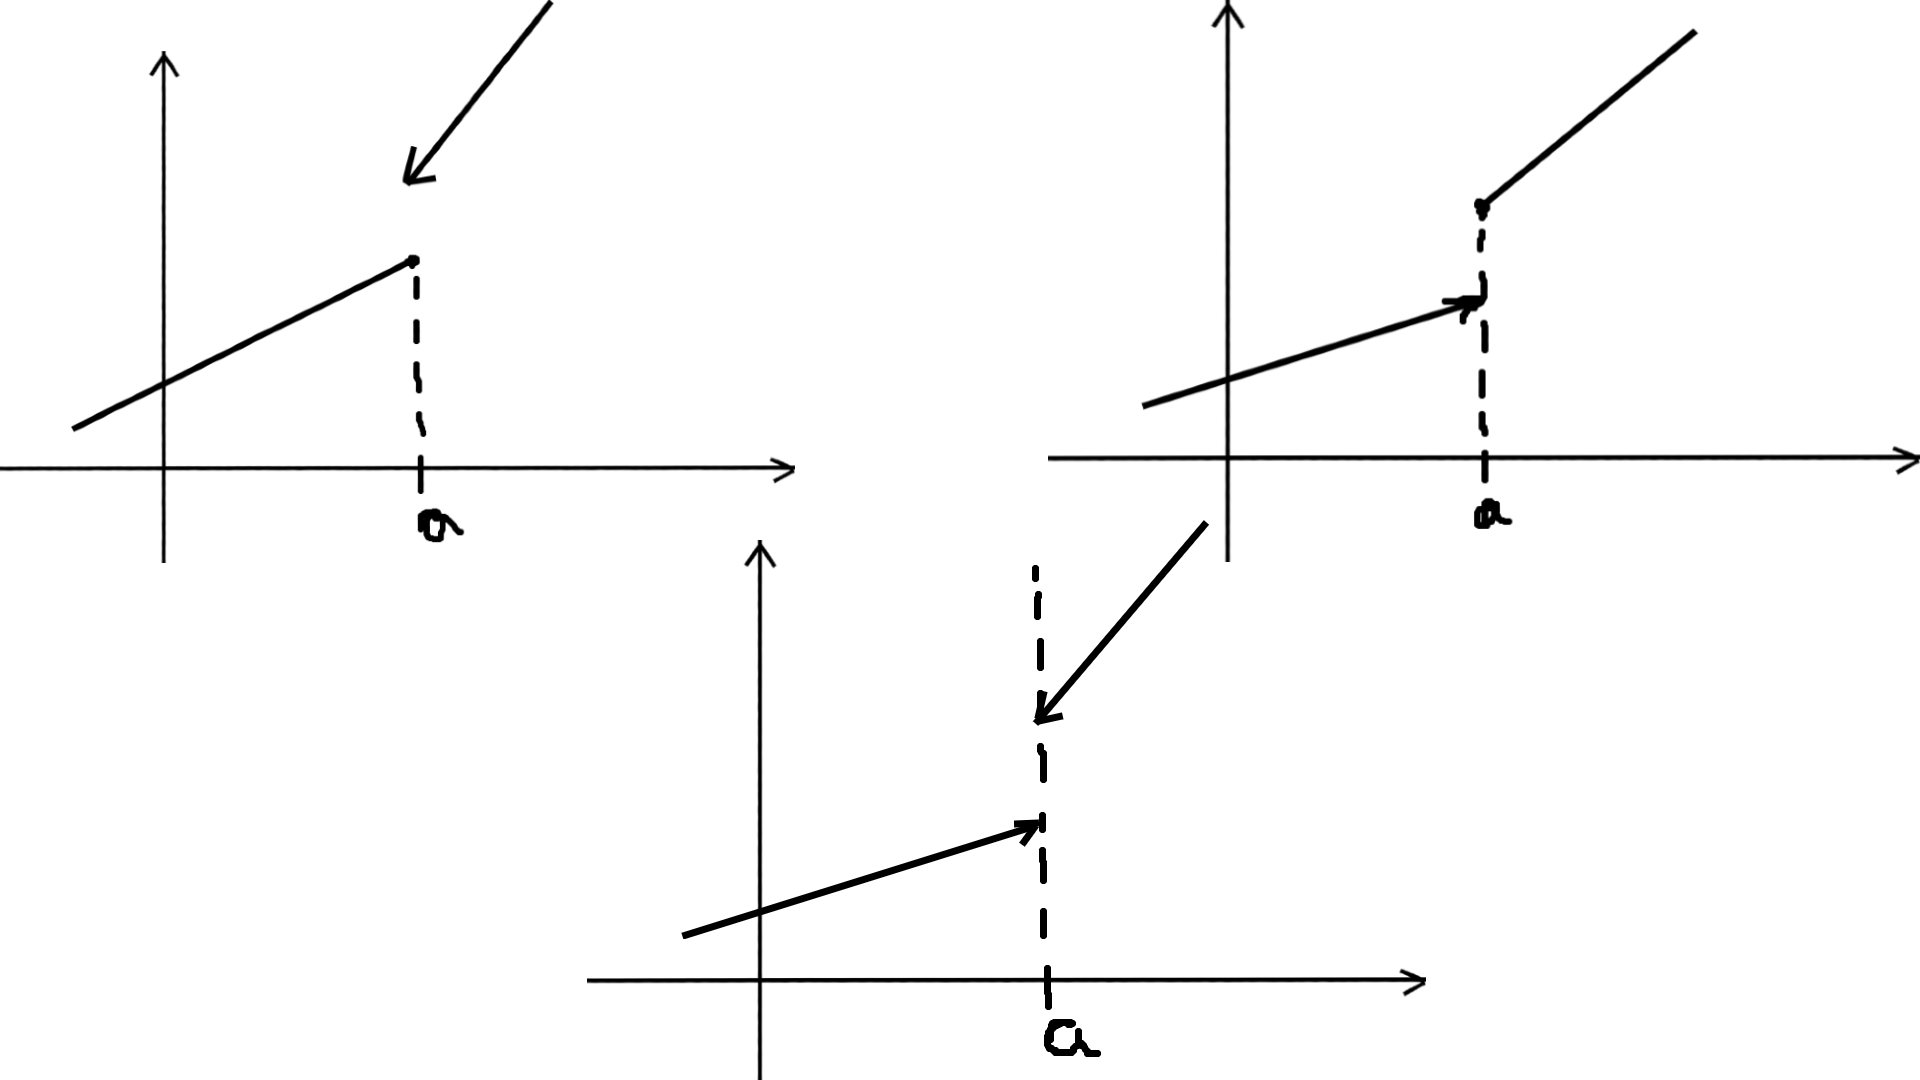
\includegraphics[width=\linewidth]{11_1_3_3.png}
        \captionof{figure}{Неустранимые разрывности}
    \end{minipage}

    \textbf{Определение.} Если в \(x=a\) функция разрывна, и этот разрыв не является разрывом первого рода, то жто разрыв 2-го рода.

    \(y = \sin \frac{1}{x}\) в \(x=0\)

    \(x_n'=\frac{2}{\pi+4\pi n} \rightarrow 0\)

    \subsection{Основные теоремы о функциях непрерывных в точке}

    \textbf{Теорема 1 (об арифметических операциях).} Пусть \(f(x)\) и \(g(x)\) непрерывны в \(x = a\), тогда 

    \begin{enumerate}
        \item \( f(x) \pm g(x) \)
        \item \( f(x) \cdot g(x) \)
        \item \( \frac{f(x)}{g(x)},\ g(a) \neq 0 \)
    \end{enumerate}
    
    1., 2., 3. --- непрерывны в \(x=a\)

    \(\uparrow\) Доказывается как следствие теоремы об арифметических операциях над пределами функций. \(\downarrow\)

    \textbf{Теорема 2.} Если \(f(x)\) непрерывна в \(x = a\), то \(\exists \delta:\ f(x)\) ограничена \(U_{\delta}(a)\)
    
    \(\uparrow\ \exists lim_{x \rightarrow a} f(x)=f(a):\ \forall \varepsilon > 0\ \exists \delta:\ \forall x\ \abs{x-a}<\delta\ \abs{f(x)-f(a)} < \varepsilon\), при \(\varepsilon = 1, \abs{f(x)}<\abs{f(a)}+1\ \downarrow\)


    \textbf{Теорема 3 (об отделимости от нуля).} Если \(f(x)\) непрерывна в \(x = a\) и \( f(a) \neq 0 \), то в \(\exists \delta:\ \forall x \in U_{\delta}(a)\)

    \begin{enumerate}
        \item \(\abs{f(x)}>\frac{\abs{f(a)}}{2}\)
        \item Если \(f(a)>0\); то \(f(x)>\frac{f(a)}{2}>0\)
        \item Если \(f(a)<0\); то \(f(x)<\frac{f(a)}{2}\)
    \end{enumerate}

    \(\uparrow\) Известно, что \(\forall \varepsilon > 0\ \exists \delta(\varepsilon):\ \forall x:\ \abs{x-a}=U_\delta(a)<\delta\ \abs{f(x)-f(a)}<\varepsilon\)

    Если \( \varepsilon = \frac{\abs{f(a)}}{2} \), то последнее неравенство 

    \( f(a) - \frac{\abs{f(a)}}{2} <_{*} f(x) <_{**} f(a) + \frac{\abs{f(a)}}{2} \)
    
    \(*\) Если \(f(a)>0 \Rightarrow f(x) > \frac{f(a)}{2}\)(п. 2 --- \(\downarrow\))\\
    \(**\) Если \(f(a)<0 \Rightarrow f(x) < \frac{f(a)}{2}\)(п. 3 --- \(\downarrow\))

    \( \abs{f(a)} - \abs{f(x)} \leq_{\star} \abs{f(x)-f(a)}<\varepsilon \)

    \( \star \) \( \abs{f(x)} > \abs{f(a)} - \frac{\abs{f(a)}}{2} = \frac{\abs{f(a)}}{2} \)(п. 1 --- \(\downarrow\))
    \(\downarrow\)

    \textbf{Суперпозиция функции:}
    
    \(\begin{cases}y = f(x);\ f:\ X \rightarrow Y\\ z = g(y);\ g:\ Y \rightarrow Z\\ h(x) = gof(x) = g(f(x));\ h:\ \widetilde{x} \rightarrow z;\ \widetilde{x} \subset x\end{cases}\)
    
    \textbf{Теорема 4 (непрерывность суперпозиции функций).} Пусть \( y = f(x) \) непрерывна в \(x = a\); а функция \( g(y) \) непрерывна в \( y = b = f(a) \), тогда \( h(x) = g(f(x)) \) непрерывна в \(x = a\).

    \(\uparrow\)
    \begin{enumerate}
        \item \( g(y) \) непрерывна в \(y = b\), т.е. \( \forall \varepsilon > 0\ \exists \delta(\varepsilon):\ \forall y:\ \abs{y - b} < \delta (=\abs{f(x) - f(a)} < \delta)\ \abs{g(y)-g(b)}<\varepsilon \)
        \item Из непрерывности \(y = f(x)\), по \(\delta(\varepsilon)\ \exists \delta_1(\delta):\ \forall x:\ \abs{x-a}<\delta_1\ \abs{f(x)-f(a)}<\delta\)
        \item В итоге по \(\forall \varepsilon > 0\ \exists \delta_1(\delta(\varepsilon)):\ \forall x:\ \abs{x - a} < \delta_1 \Rightarrow_{\textrm{п. 2}} \abs{f(x) - f(a)} < \delta \Rightarrow_{\textrm{п. 1}} \abs{g(f(x)) - g(f(a))} < \varepsilon\)
        
        А \( \abs{g(f(x)) - g(f(a))} < \varepsilon = \abs{h(x) - h(a)} < \varepsilon \)    
    \end{enumerate}
    \(\downarrow\)

    \textbf{Теорема 5.} \(y=f(x)\) определена в окрестности \(x=a\), непрерывна в \(x=a\) и обратима в окрестности \(x=a\), то обратная функция \(x = f^{-1}(y)\) непрерывна в \(y=f(a)\).
    
    \subsection{Непрерывность некоторых функций}
    
    \begin{enumerate}
        \item \( y=c=const \) непрерывна \( \forall x \)
        
        \( \forall \varepsilon > 0\ \exists \delta:\ \abs{x - a} < \delta \abs{f(x) - f(a)} = \abs{c - c} = 0 < \varepsilon \)

        \item \(y=x\) непрерывна \(\forall x\)
        
        \(\forall \varepsilon > 0\ \exists \delta:\ \abs{x - a} < \delta \abs{f(x) - f(a)} = \abs{x - a} < \delta = \varepsilon\)
    
        \(y=x^n\) непрерывна \(\forall x\), как произведение непрерывных функций
        
        \item \(y = a_n x^n + a_{n-1}x^{n-1}+...+a_1x+a_0 = P_n(x)\) непрерывна \(\forall x \in \mathbb{R}\) как \(\pm;\ a_i \in \mathbb{R}, n \in \mathbb{N}\)
    
        \item \( y = \frac{P(x)}{Q(x)} = \frac{a_{n}x^{n} + a_{n - 1}x^{n - 1} + ... + a_0}{a_{m}x^{m} + a_{m - 1}x^{m - 1} + ... + a_0} \)
        
        Непрерывна \(\forall x,\ Q(x) \neq 0\)
            
        \item \(y = sin\ x\)

        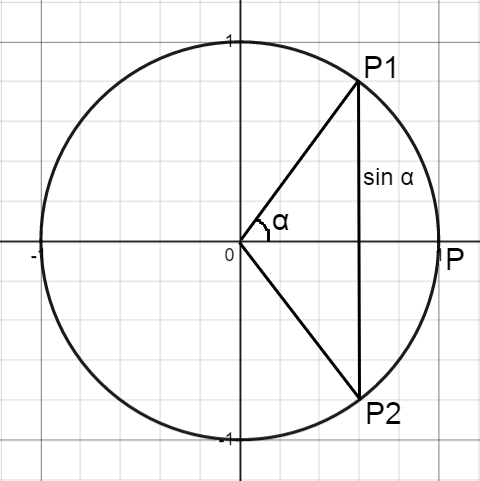
\includegraphics[scale=0.35]{11_1_3_4.png}

        \( \abs{sin\ \alpha} \leq \abs{\alpha} \)

        \begin{enumerate}
            \item \(0 < \abs{\alpha} \leq \frac{\pi}{2}\)

            \(\abs{P_1P_2}=2\abs{sin\ \alpha}\)

            \( P_1PP_2 = 2\abs{\alpha}\)
            
            \(\abs{P_1P_2}<P_1PP_2 \Rightarrow \abs{sin\ \alpha} < \abs{\alpha}\)

            \item при \( \alpha = 0 \), равенство
            \item \( \abs{\alpha} > \frac{\pi}{2}\ \abs{sin\ \alpha} \leq 1 < \frac{\pi}{2} < \abs{\alpha} \)
            
            \( \forall \varepsilon > 0\ \exists \delta:\ \forall x \abs{x - a} < \delta \Rightarrow \abs{sin\ x - sin\ a} < \varepsilon \)
            
            \(\abs{sin\ x - sin\ a} = \abs{2sin\frac{x-a}{2}cos\frac{x+a}{2}} = 2\abs{sin\frac{x - a}{2}}\abs{cos\frac{x + a}{2}} < 2 * \frac{\abs{x - a}}{\abs{2}} * 1 < \delta = \varepsilon\)
        \end{enumerate}

        \item \(y = cos\ x\) непрерывна \(\forall x\)        
        \item \(y = \abs{x}\)

        \(\abs{f(x)-f(a)} = \abs{\abs{x}-\abs{a}} \leq_* \abs{x-a} < \delta = \varepsilon\)

        \(*\ \abs{x}-\abs{a} \leq \abs{x-a}\)
        
        \(\abs{a}-\abs{x} \leq \abs{x-a}\)

        \(-\abs{x-a} \leq \abs{x} - \abs{a} \leq \abs{x-a}\)

        \item \( y = sin^5\ x^2 \) непрерывна как "комбинация" непрерывных функций
        \item \( y = x^2 (x \geq 0) \rightarrow y = \sqrt{x} \) 
    \end{enumerate}
\end{document}
